\documentclass[aps,prb,10pt,twocolumn,groupedaddress]{revtex4-1}
%\setlength\topmargin{4.6mm}
%\documentclass{[prl,twocolumn]{revtex4-1}
%\usepackage[ansinew]{inputenc}
%\usepackage[latin1]{inputenc}% PROPER ENCODINGS
%\usepackage[T1]{fontenc}%      FOR FINNISH TEXT
%\usepackage[finnish]{babel}% 
%\usepackage[official]{eurosym}

%\usepackage{subfig}
\usepackage{caption}
\usepackage{subcaption}
\usepackage{graphicx}
\usepackage{epsfig}
\usepackage{epstopdf}
\usepackage{amsmath}
\usepackage{blkarray}
\usepackage{multirow}
\usepackage{mathtools}
\usepackage[font=small,labelfont=bf]{caption}

%\usepackage{subfig}
%\usepackage[footnotesize]{caption}
%\pagestyle{empty}
%\setlength{\textwidth}{140mm}
%\setlength{\textheight}{240mm}
%\setlength{\parindent}{0mm}
%\setlength{\parskip}{3mm plus0.5mm minus0.5mm}
\bibliographystyle{apsrev4-1}
%%%%%%%%%%%%%%%%%%%%%%%%%%%%%%%%%%
\begin{document}

\title{Automatic Detection of Blood Vessels From Retinal Images Using Convolutional Neural Network }
\date{\today}
\author{Ville Virkkala, Jarno Leppänen}
\affiliation{Ekahau Research}

\begin{abstract}
  
\end{abstract}

\maketitle

\section{Introduction}

Several studies have used neural networks in automatic blood vessel detection from retinal images. These methods can be roughly divided into two groups: patch based segmentation of blood vessels and methods based on fully convolutional neural networks. In patch based image segmentation the image is traversed through pixel by pixel. For each pixel a patch of fixed size, centered at the pixel, is taken from the image and fed to neural network that classifies the pixel into certain class.
The advantages of patch based method are their simplicity and ease of training. However, their main disadvantage is the high computational load when doing inference, because for each pixel separate patch is taken that is fed to neural network. Fully convolutional neural network are the current state of the art method in image segmentation. The huge advantage of fully convolutional neural network is the huge speed up compared to patch based methods, because the whole image is fed only once as whole to the neural network. In addition there is more contextual information available in fully convolutional neural networks because the whole image is processed at once instead of using smaller patches. 

In this work patch based semantic segmentation method using convolutional neural network is developed to detect blood vessels from retinal images. The performance of the developed method is validated against several test images. In addition performance of the developed method is compared to random forest classifier implemented in scikit-learn python library.
The paper is organized as follows. The used data-set and the computational
methods are described in detail in sections \ref{sec:used_data_set} and \ref{sec:methods}. In Sec. \ref{sec:results} training metrics and performance of the developed method in inference when applied on test images are given.
Sec. \ref{sec:conclusions} is a summary of the results and the differences between the two classifiers are discussed.

\section{Used data-set}
\label{sec:used_data_set}
The used data set in this work is the publicly available DRIVE data set \cite{drive} available in \cite{drive_url}. The data set consist of 40 images of size 565x584 and the corresponding ground truth annotations of blood vessels. The images were obtained from diabetic subjects as a part of diabetic retinopathy screening program in The Netherlands.

The data set was divided into training, validation and test sets containing 28, 6 and 6 images respectively. The images are three channel RGB images, but only the green channel was used in classification, because typically the blood vessels are best visible at the green channel. In classification of pixels patches of size 33x33 centered at the pixel were used. Examples of retinal image that is classified and the corresponding ground truth image are shown in figures \ref{fig:example_images}a and \ref{fig:example_images}b respectively. Examples of patches that corresponds to pixels that are labeled as blood vessels and background are shown in figures \ref{fig:example_patches}a-\ref{fig:example_patches}c and \ref{fig:example_patches}d-\ref{fig:example_patches}f respectively.
\begin{figure*}[!t]
	\centering
	\begin{subfigure}[]{0.4\textwidth}
		\centering
		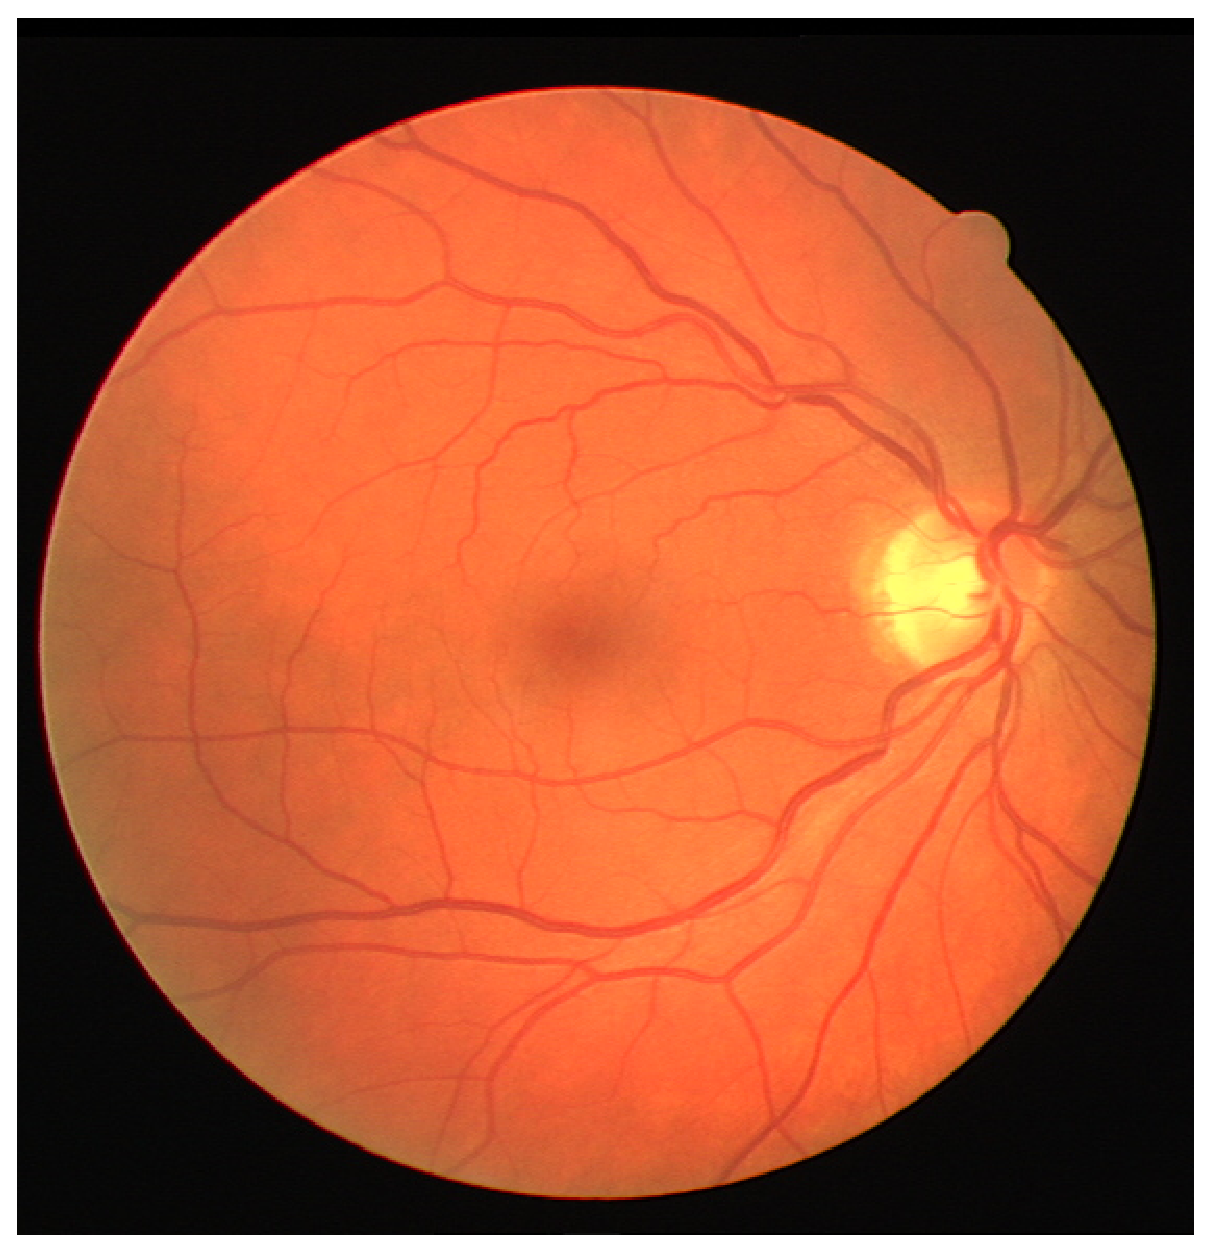
\includegraphics[width=\textwidth]{images/02_training.eps}
		\caption{}
	\end{subfigure}
	\hspace{1cm}
	\centering
	\begin{subfigure}[]{0.4\textwidth}
		\centering
		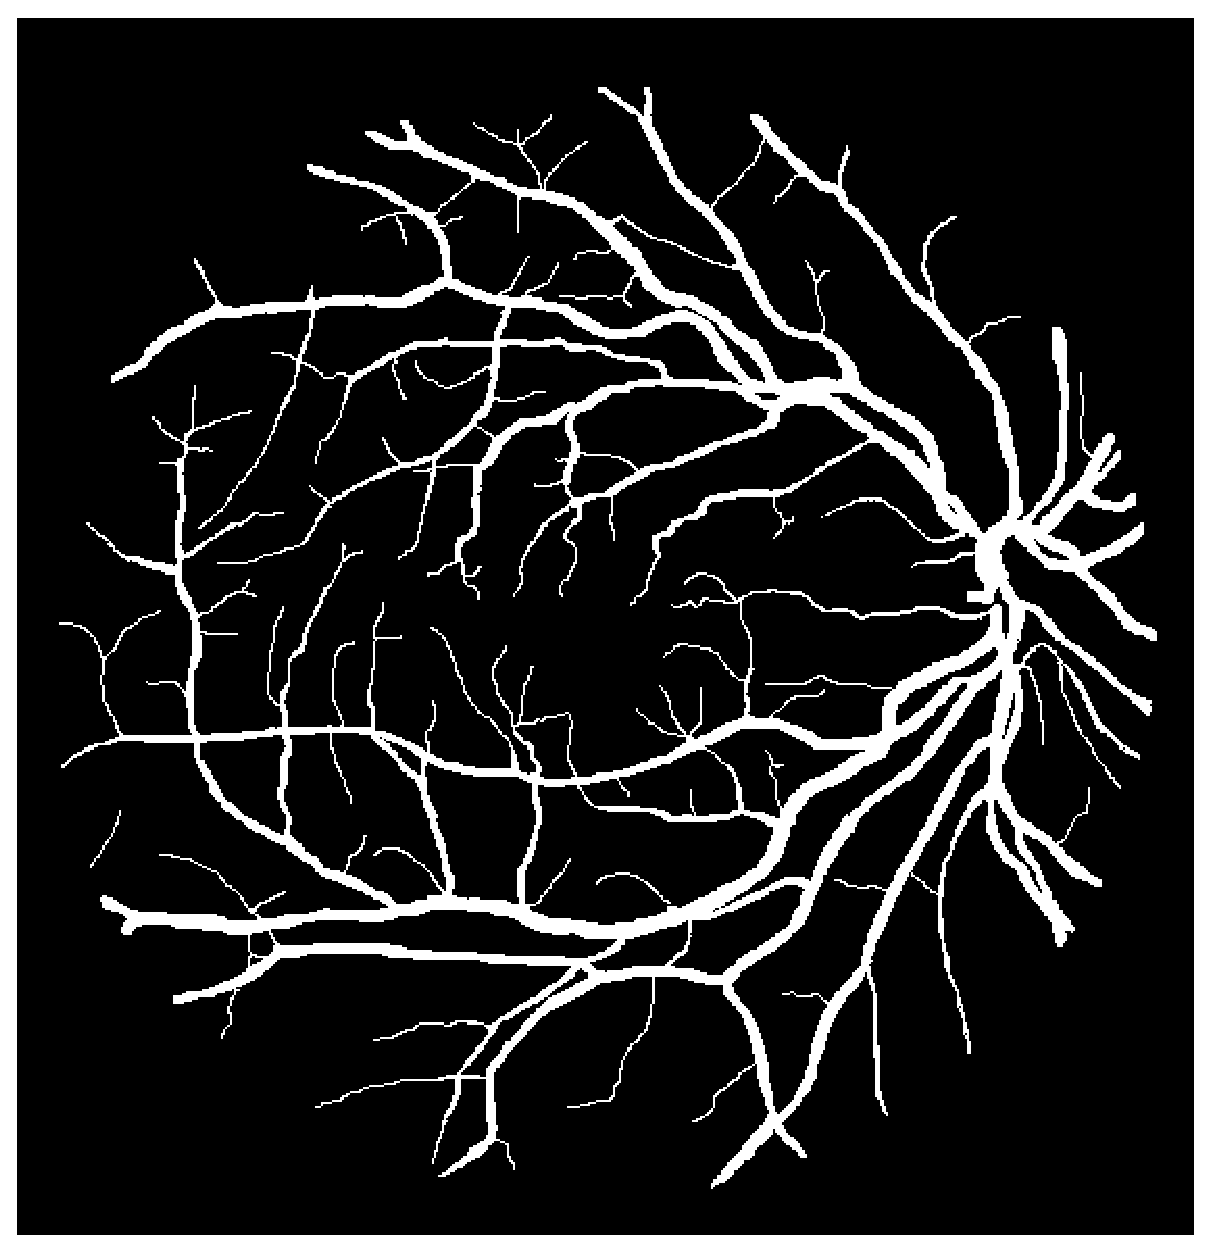
\includegraphics[width=\textwidth]{images/02_manual1.eps}
		\caption{}
	\end{subfigure}\\
	\caption{Example of retinal image used in training (a) and the corresponding ground truth annotation of blood vessels (b).}
	\label{fig:example_images}
\end{figure*}

\begin{figure*}[!b]
	\centering
	\begin{subfigure}[]{0.25\textwidth}
		\centering
		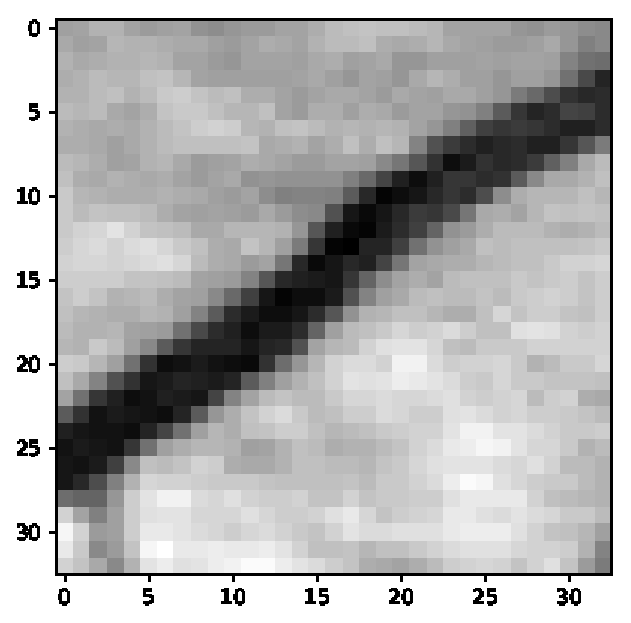
\includegraphics[width=\textwidth]{images/positive1.eps}
		\caption{}
	\end{subfigure}
	\hspace{0.75cm}
	\centering
	\begin{subfigure}[]{0.25\textwidth}
		\centering
		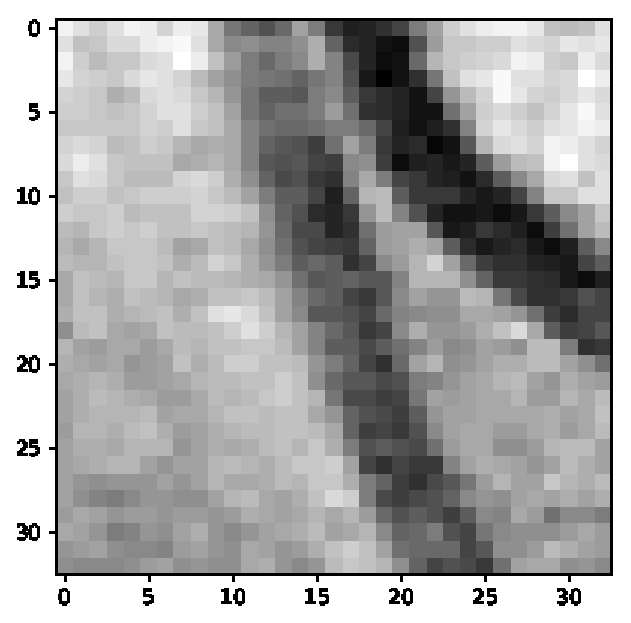
\includegraphics[width=\textwidth]{images/positive2.eps}
		\caption{}
	\end{subfigure}
	\hspace{0.75cm}
	\centering
	\begin{subfigure}[]{0.25\textwidth}
		\centering
		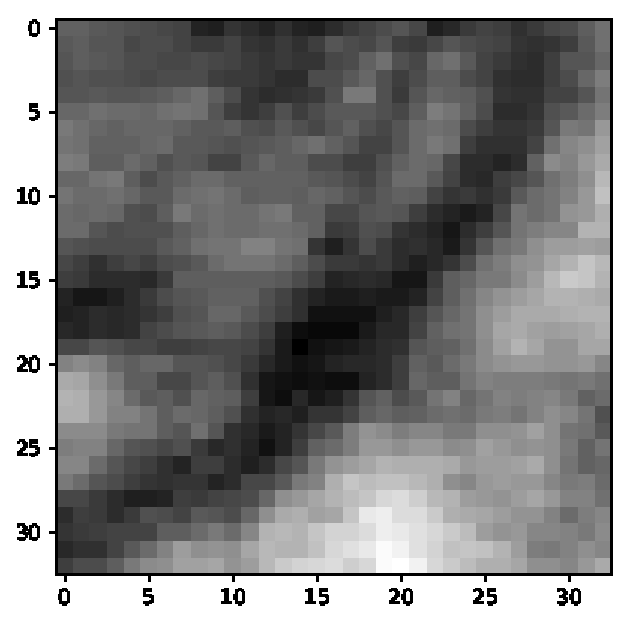
\includegraphics[width=\textwidth]{images/positive3.eps}
		\caption{}
	\end{subfigure}\\
	\vspace{0.75cm}
	\centering
	\begin{subfigure}[]{0.25\textwidth}
		\centering
		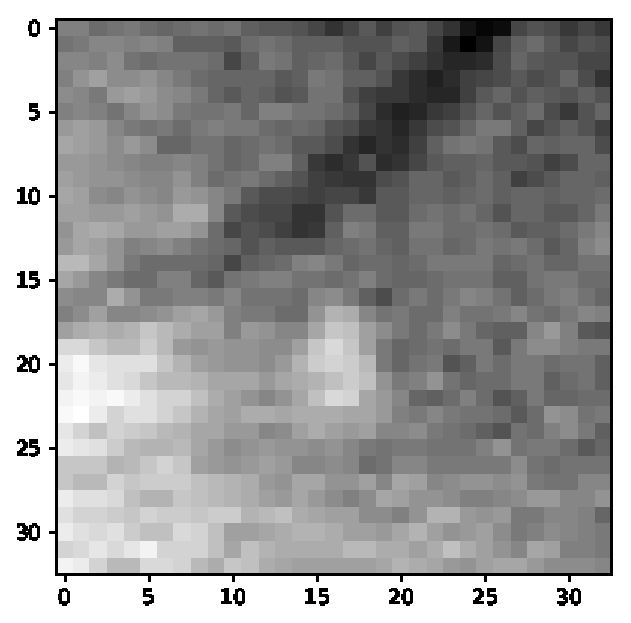
\includegraphics[width=\textwidth]{images/negative1.eps}
		\caption{}
	\end{subfigure}
	\hspace{0.75cm}
	\centering
    \begin{subfigure}[]{0.25\textwidth}
    	\centering
    	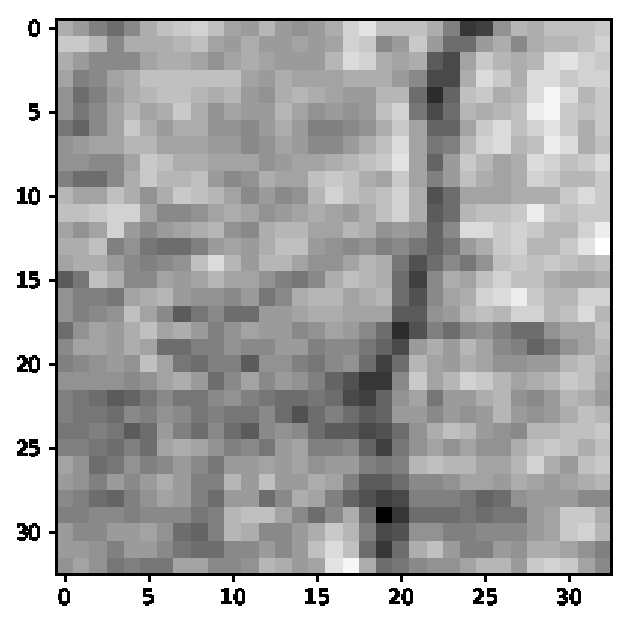
\includegraphics[width=\textwidth]{images/negative2.eps}
    	\caption{}
    \end{subfigure}
    \hspace{0.75cm}
    \centering
    \begin{subfigure}[]{0.25\textwidth}
    	\centering
    	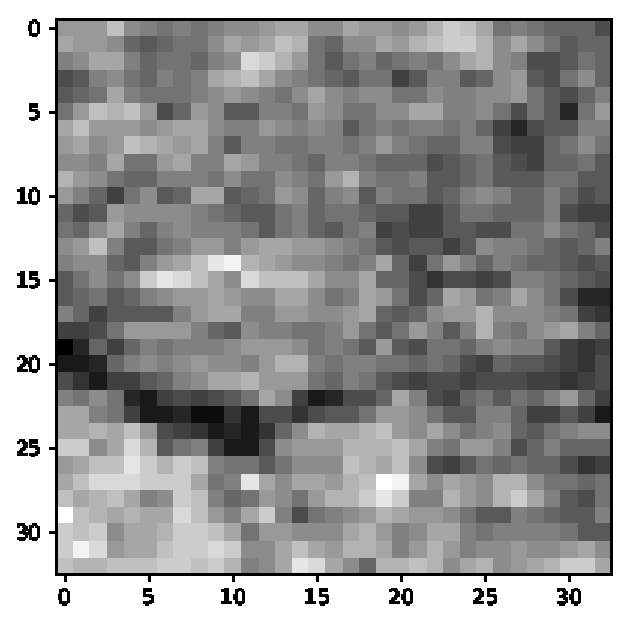
\includegraphics[width=\textwidth]{images/negative3.eps}
    	\caption{}
    \end{subfigure}\\
	\caption{Examples of patches corresponding to pixels that are labeled as blood vessels (a)-(c) and patches corresponding to pixels that are labeled as background (d)-(f). The pixel that the label is related to is located at the center of patch.}
	\label{fig:example_patches}
\end{figure*}


\section{Computational methods}
\label{sec:computational_methods}
In this work two different methods were used to classify the songs to different
genres. First method is logistic-regression method in which the logistic-loss
is minimized iteratively using the gradient descent method.
The other method used is the Bayes-classifier which classifies the song to
certain category that gives the maximum posterior probability with respect to
label $i$. Both methods are described below in detail. In addition we studied
the effect of feature extraction and for that purpose we used principal
component analysis method to exclude features with little impact. 
\subsection{Developed Convolutional Neural Network}
\label{sec:computational_methods_developed_network}

\subsection{Training}
\label{sec:computational_methods_training}
The developed method above contains three hyper parameters, the number of kernels in first and second convolution layer and the number of layers in first fully connected layer. Rest of the parameters, \textit{i.e.}, the kernel size and patch size were kept fixed. The optimal hyper parameters were found using random search. Ten different configurations were randomly sampled from given intervals that were $\lbrack$10, 35$\rbrack$, $\lbrack$10, 35$\rbrack$ and $\lbrack$200, 1200$\rbrack$ respectively for the hyper parameters. For each configuration the network was trained over 125 samples. In addition an early stopping criterion, evaluated against the test set, with tolerance of 0.01 and patience of 2 was used to avoid over fitting of the model. Adam optimizer\cite{adam} initialized with learning rate $1e-6$ was used to optimize the network parameters in back propagation. The final accuracy of the network, with given hyper parameters, was then obtained evaluating the accuracy against the test set. Final network, used in inference, was then constructed using the hyper parameters corresponding to best accuracy obtained. The final network was then retrained over 250 epochs or until early stop to get full convergence.

\subsection{Inference}
\label{sec:computational_methods_inference}

\section{Results}
\subsection{Optimal hyper parameters and the training accuracy}
\label{sec:results_training}
The results for the hyper parameter search, explained in section \ref{sec:computational_methods_training}, are shown in Table \ref{tab:hyperparameter_searach_accuracies}. According to Table \ref{tab:hyperparameter_searach_accuracies} the best accuracy was obtained when the hyper parameters were set to 33x67x355. The final accuracy with these parameters for test set, after training over 250 epochs was 0.84\%. The validation accuracy with respect to epoch number is shown in figure \ref{fig:validation_accuracy}.
\begin{center}
	\begin{table}[b]
		\begin{tabular*}{0.45\textwidth}{lclc}
			Configuration & Accuracy (\%) & Configuration & Accuracy (\%)\\
			\hline
			33x67x355 & 83.8 & 16x50x981 & 82.9\\
			29x42x709 & 83.7 & 18x63x1048 & 82.9\\
			29x49x871 & 83.5 & 27x58x359 & 82.4\\
			19x57x1158 & 83.3 & 10x64x1176 & 81.3\\
			20x60x256 & 83.2 & 14x49x638 & 80.1\\
		\end{tabular*}
		\caption{Results of the random hyper parameter search. The numbers in the configuration column indicates the number of kernels in the first and second convolution layers and the number of neurons in the first fully connected layer respectively. The accuracy is obtained running the trained network with the given hyper parameters against the test data set.}
		\label{tab:hyperparameter_searach_accuracies}
	\end{table}
\end{center}

\section{Conclusions}
\label{sec:conclusions}
In this work we used logistic-regression and Bayes-classifier to classify songs
to different genres based on the music signal's characteristics. For logistic
regression the obtained accuracy for test set was 0.67 and logistic-loss 0.27.
For the external data set used the obtained accuracy and logistic-loss were 0.65
and 0.178 respectively in the case of logistic-regression. For the
Bayes-classifier the obtained accuracy and logistic-loss were 0.53 and 0.33 for
the test-data and for external data set 0.32 and 1.17 respectively. According to
obtained results both classifiers performed clearly better than random guess,
but remained far from perfect classification. From the two classifiers used
the logistic-regression classifier performed clearly better. The logistic
classifier also generalized much better to completely new data giving nearly
equal performance for test data set and external data set.

\bibliography{references}

\end{document} 






